\documentclass[11pt, letter, margin = 2 in]{article}

\usepackage[style = authoryear, autocite=inline, doi=false,isbn=false,url=false]{biblatex}
\usepackage[colorlinks, citecolor = red]{hyperref}
\usepackage[long, nodayofweek]{datetime}
\usepackage[]{booktabs}
\usepackage{graphicx}

\usepackage[sf,pagestyles]{titlesec} % make section headings \sffamily
% make headers \sffamily
\newpagestyle{main}[\sffamily]{
    \sethead{\thepage}{}{\sectiontitle}
    }
\pagestyle{main}
\usepackage{titling}
% make titling elements \sffamily
\pretitle{\begin{center}\sffamily\LARGE}
\preauthor{\begin{center}
            \large\sffamily \lineskip 0.5em%
            \begin{tabular}[t]{c}}
\predate{\begin{center}\sffamily\large}
\usepackage{abstract}
% make abstract title \sffamily
\renewcommand\abstractnamefont{\sffamily}
\usepackage{caption} 
\captionsetup{font=sf, labelfont = bf}

\begin{document}
\author{Andy Eggers\thanks{Nuffield College and Department of Politics and International Relations, University of Oxford, United Kingdom. \texttt{aeggers@nuffield.ox.ac.uk}}
\and
Tobias Nowacki\thanks{Department of Political Science, Stanford University, CA, United States. \texttt{tnowacki@stanford.edu}}}
\date{\today}
\title{Checking Theory Predictions}

\maketitle

\begin{figure}[!htb]
	\centering
	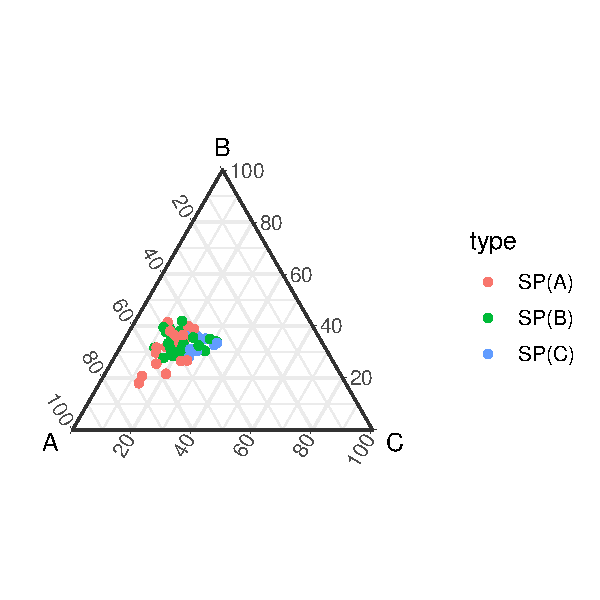
\includegraphics[width = .6\textwidth]{../output/figures/prediction/sp_cases_tern.pdf}
	\caption{Distribution of first preferences of all single-peaked cases}
	\label{fig:figure1}
\end{figure}


For each of the different classes, I will present two plots: one is the distribution of pivotal probabilities (by event) within that class, and the other one is the distribution of strategic votes (by permutation) within that class.\footnote{Note that I decided against plotting second-round pivotal probabilities here because they are much larger in relative terms and would render comparisons between first-round ones unreadable.} In the latter, the colours refer to Table 3 in Andy's Theory memo: \textbf{orange} means that this is a confident prediction (black text); \textbf{light grey} denotes those with moderately likely second-round events (grey text); and \textbf{dark grey} denotes those that are crossed out.

Note that this exercise does not involve any analysis of preference intensity -- $\beta$'s are just taken as given from the data.

\section{Single-Peaked}

\subsection{A is the attractor}

\begin{figure}[!htb]
	\centering
	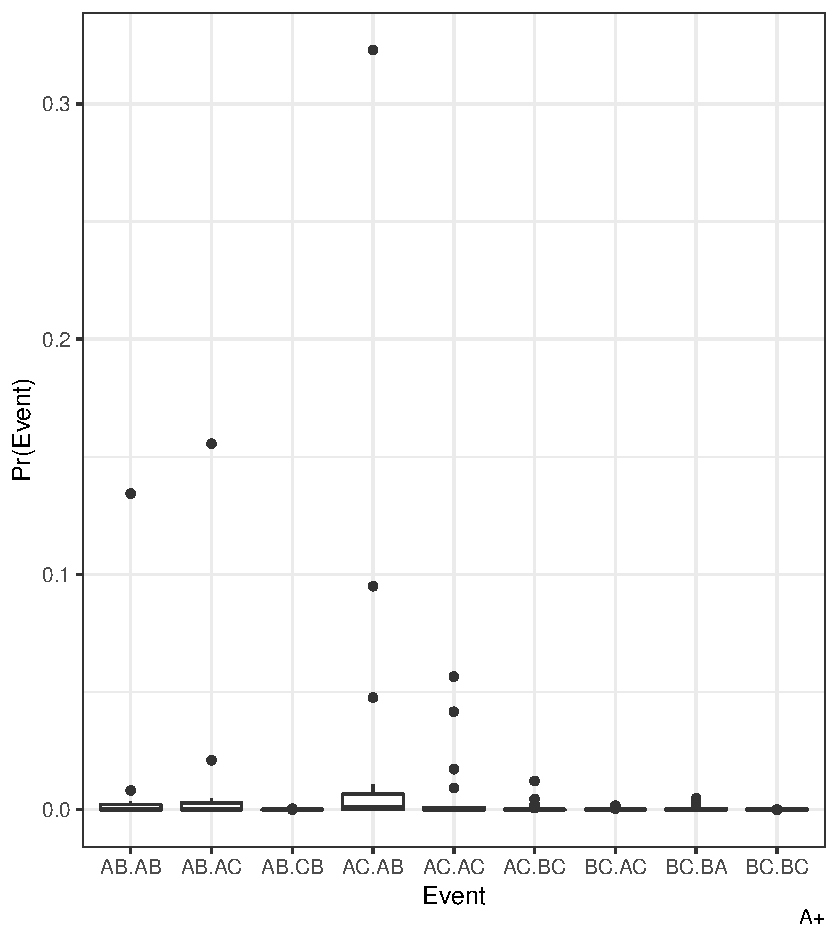
\includegraphics[width = .45\textwidth]{../output/figures/prediction/pprob_sp_a.pdf}
	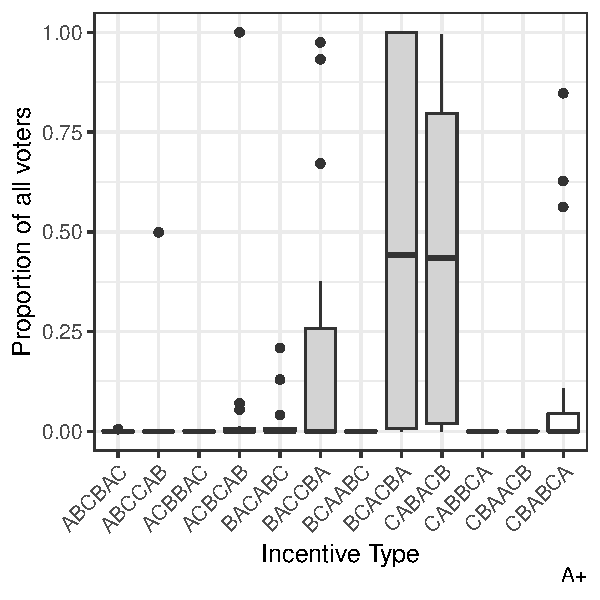
\includegraphics[width = .45\textwidth]{../output/figures/prediction/svinc_sp_a.pdf}
	\caption{Distribution of pivotal probabilities and proportions of strategic vote incentives for all $A+$ cases.}
	\label{fig:figure1}
\end{figure}

The theoretical prediction is that $AC.AB$ is the dominant pivotal event; this holds true in the empirical data. However, there are a few outliers with high probabilities for $AC.AC$ in particular, and a few for $AC.BC$. (Need to check whether $AB.XX$ events are non-trivial here). 

Consequently, the $CAB \rightarrow ACB$ strategic incentive is high. The $BCA \rightarrow CBA$ strategic incentive would only be attenuated by a high likelihood of $BC$ events in the second round; however, this does not seem to be the case and thus the $BCA \rightarrow CBA$ incentive is also very strong. Finally, the $BAC \rightarrow CBA$ incentive is attenuated by both $BC$ \textit{and} $AC$ and occurs much rarer. Note that the mean levels of strategic incentive proportions for $CAB \rightarrow ACB$ and $BCA \rightarrow CBA$ are much lower than for the $B+$ and $C+$ cases -- this is because, in relative terms, the $AC.AB$ event is much less likely than the $BC.XX$ ones.

\subsection{B is the attractor}

This is the old case of B having neutral preferences and A, C voters both choosing B in second preferences.

\begin{figure}[!htb]
	\centering
	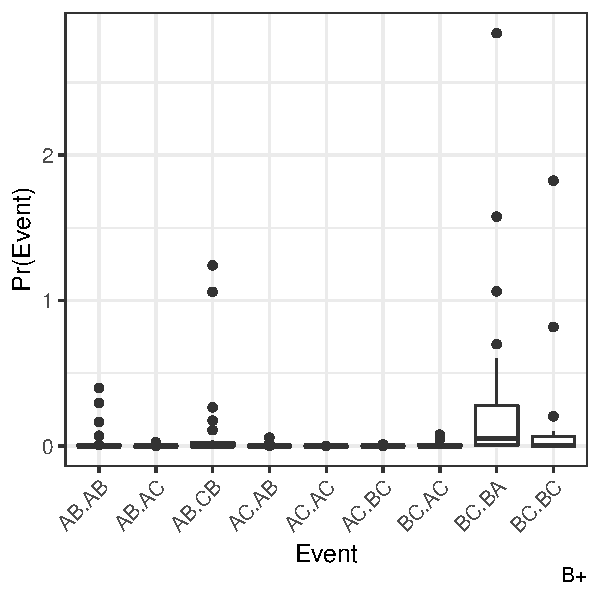
\includegraphics[width = .45\textwidth]{../output/figures/prediction/pprob_sp_b.pdf}
	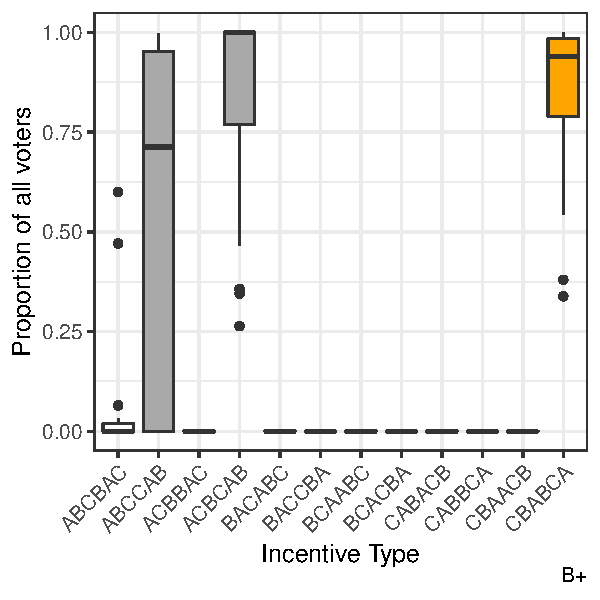
\includegraphics[width = .45\textwidth]{../output/figures/prediction/svinc_sp_b.pdf}
	\caption{Distribution of pivotal probabilities and proportions of strategic vote incentives for all $B+$ cases.}
	\label{fig:figure1}
\end{figure}

As predicted by the theory, the $BC.BA$ pivotal event clearly dominates here, with $BC.BC$ coming second.

Unsurprisingly, this means that the incentive to vote $CBA \rightarrow BCA$ is very high -- in only two cases have less than half of all $CBA$ voters an incentive to follow this insincere vote. However, the proportion of $ACB \rightarrow CAB$ incentives is also very high (in fact, the mean is even higher!). This is because the likelihood of a conflicting $AC$ event in the second round is extremely small (given our labelling of the parties). Graphically, it seems that the majority of our $B+$ cases also have $B$'s second preferences slightly tilt to the right, which (I think) decreases the probability of this vote type "backfiring". Finally, the $ABC \rightarrow CAB$ incentive is, again, somewhat lower, and experiences a lot more variance than the others, because of the additional consideration of the (more likely) $BC$ second-round event. 

Here, the prediction for the crossed out elements does not appear to hold, because in the empirics, the second-round pivotal events appear to be much less likely.

\subsection{C is the attractor}

\begin{figure}[!htb]
	\centering
	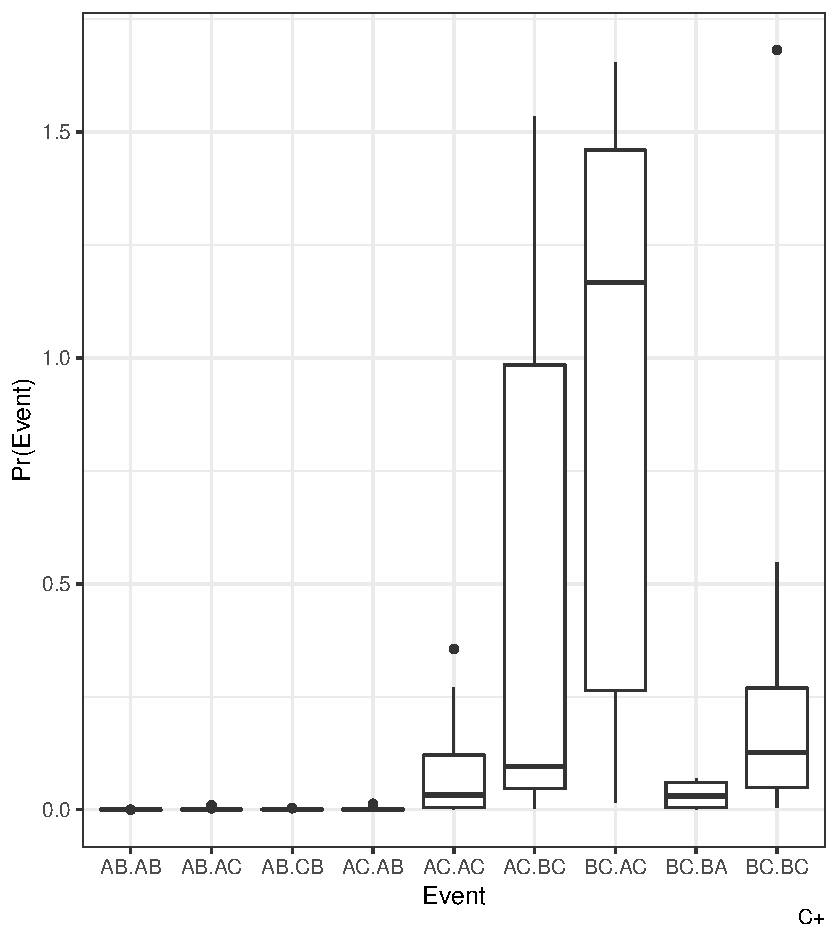
\includegraphics[width = .45\textwidth]{../output/figures/prediction/pprob_sp_c.pdf}
	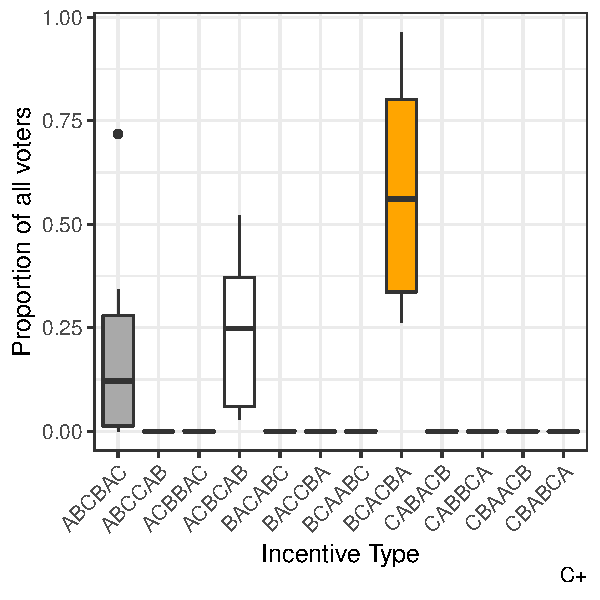
\includegraphics[width = .45\textwidth]{../output/figures/prediction/svinc_sp_c.pdf}
	\caption{Distribution of pivotal probabilities and proportions of strategic vote incentives for all $C+$ cases.}
	\label{fig:figure1}
\end{figure}

Here, the $BC.AC$ event is clearly the dominant one, however, we see a few others ($AC.AC$, $AC.BC$, $BC.BC$) that are also relevant. Consequently, because of the high $BC.AC$ probability, the predicted $BCA \rightarrow CBA$ incentive is also the most prevalent one. There is also some incidence of the $ABC \rightarrow BAC$ incentive, which would only be mitigated by the $AB$ second-round pivotal event (which is quite likely, no?). Surprisingly, $ACB$ voters appear to have some incentive to vote $\rightarrow CAB$. This is probably because of the high probablity of $AC.BC$: here, a sincere vote would help elect the least preferred candidate (no-show). Thus, if C is the attractor, the predictions don't hold as well.

\begin{figure}[!htb]
	\centering
	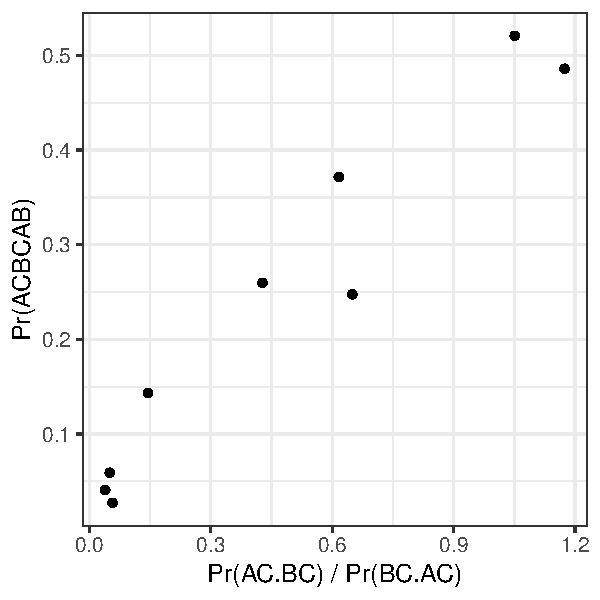
\includegraphics[width = .45\textwidth]{../output/figures/prediction/sp_c_odd.pdf}
	\caption{Proportion of $ACB$ voters with incentive to vote $CAB$ by the probability of the $AC.BC$ pivotal event relative to $BC.AC$.}
	\label{fig:figure1}
\end{figure}

\section{Divided Majority}


\end{document}